\chapter{PMD}\label{ch:pmd}

PMD is a static source code analyzer. This tool looks at Java source code and identifies bugs or potential anomalies. These anomalies include dead code, duplicated code or overcomplicated expressions \cite{Urma}.

The first version of PMD (version 0.1) was introduced in 2002. The version of PMD that was used in this project is 5.4.1. 

PMD can check for more that plain java program issues. Its rules are divided into 5 sections: jsp, xsl, java, ecmascript, and xml. In the java section there are 276 different checks divided into 16 categories: Design (52), Coupling (10), Jakarta Commons Logging (3), Basic (23), Strict Exceptions (12), Security Code Guidelines (2), Java Logging (4), Android (3), Controversial (23), Comments (3), Type Resolution(4), Empty Code(11), String and StringBuffer (15), Code Size (11), Braces (4), Unused Code (5), Unnecessary (7), J2EE (9), JavaBeans (2), Migration (14), Import Statements (6), JUnit (12), Naming (20), Finalizer (6), Optimization(12), and Clone Implementation(3). The number in parenthesis marks the number of checks in that category. The rules range from styling checks like ``ShortMethodName: Method names that are very short are not helpful to the reader" in the Naming category to rules for checking code design like ``UseSingleton: For classes that only have static methods, consider making them Singletons. Note that this doesn't apply to abstract classes, since their subclasses may well include non-static methods. Also, this class is a Singleton, a private constructor should be added to prevent instantiation."

From the rule sets PMD uses, it is able to assist programmers in finding logic based bugs. Some of the categories that may be able to identity potential bugs include Controversial, Empty Code, and String and StringBuffer. One of the rules in the category, Controversial that may cause a logic based bugs is the UnnecessaryParantheses. UnnecessaryParantheses is using the order of operation to calculate a certain math equation, and parantheses that are used may lead to an incorrect answer. In the category Empty Code, one ruleset that may lead to logic based bugs is EmptyCatchBlock. If the catch block is empty, then nothing will be done which could cause an incorrect calculation. In the category of String and StringBuffer, one ruleset that caused a logic based bug was the UseEqualsToCompareStrings. In this ruleset, if two string are compared in an if statement by using ==, this is not going to work correctly. This is because the == operator looks at what the string point to rather than the content of the strings. To fix this, the .equals() method should be used to compare two strings.

Comparing FindBugs and PMD, PMD has found to produce a larger amount of warnings than FindBugs. Despite that more warnings in a piece of source code will be generated with PMD compared to FindBugs, this does not mean that FindBugs or PMD is the better tool. These two tools focus on two different aspects of software quality \cite{Hovemeyer:2004:FBE:1028664.1028717}. PMD focus on looking at a coding style. FindBugs focuses on helping to uncover errors while ignoring style issues. Since these two tools focus on two different aspects of software quality, these two tools are complements of each other and not substitutes.

\newpage
\begin{figure}
\begin{center}
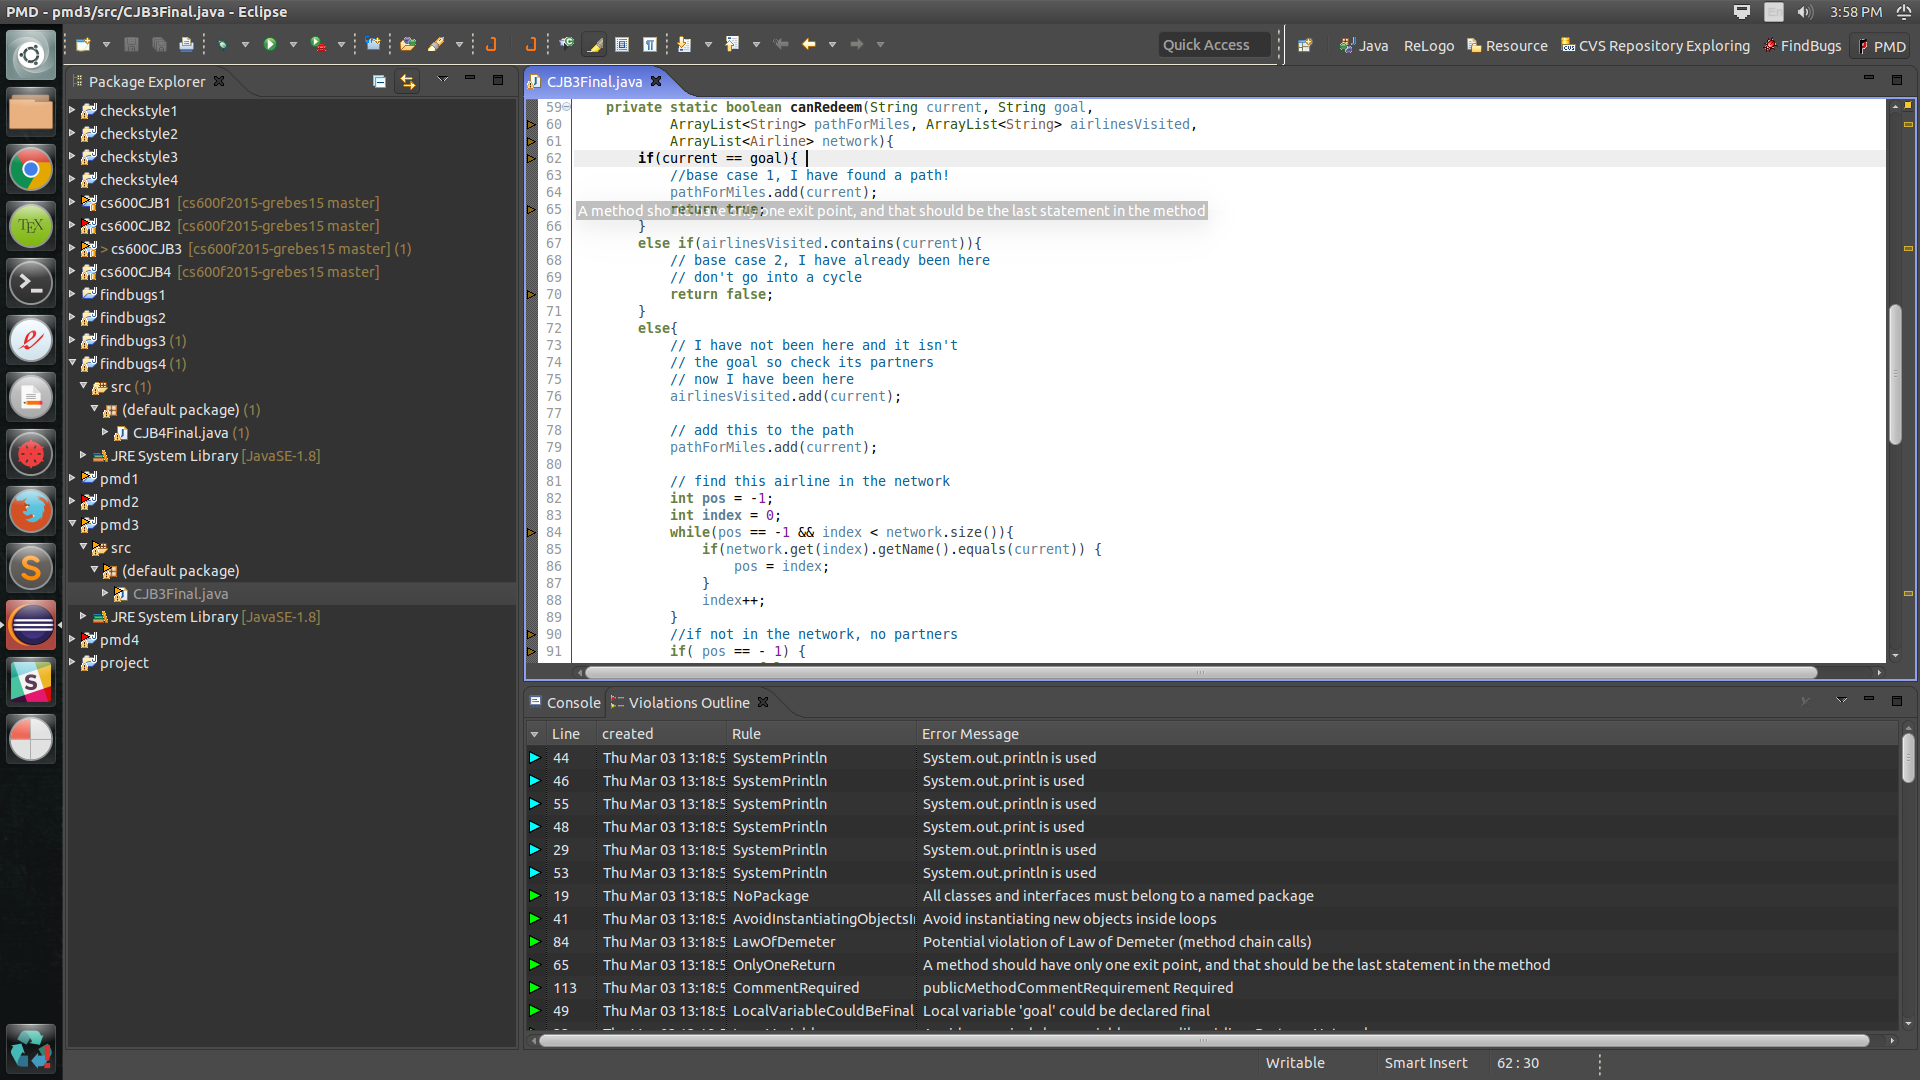
\includegraphics[width=1.15\textwidth]{pmd.png}
\end{center}
\caption{Example of PMD used in the Eclipse Integrated Development Environment}
\label{fig:pmd}
\end{figure}
Figure \ref{fig:pmd} is a screenshot taken that shows the PMD tool used in the empirical study. Inside of the Eclipse Integrated Development Environment, PMD highlights multiple lines of source code and displays a warning. All of the highlighted lines can be seen on the left side of the line numbers.   

\section{AST - Abstract Syntax Tree}
\label{sec:ast}

An Abstract Syntax Tree is an tree representation of the source code. This tree can be viewed as a structured document - just like XML. Since it is  conceptually similar to XML, it can be queried with XPath to find a pattern \cite{pmd}. By having the source code represented as a tree means the checks can be made at isolated nodes in the tree, irrespective of branches higher up and below. The Abstract Syntax Tree shows the structure of the code - the blocks and statements that are contained within each element.

\begin{figure}[H]
\begin{center}
	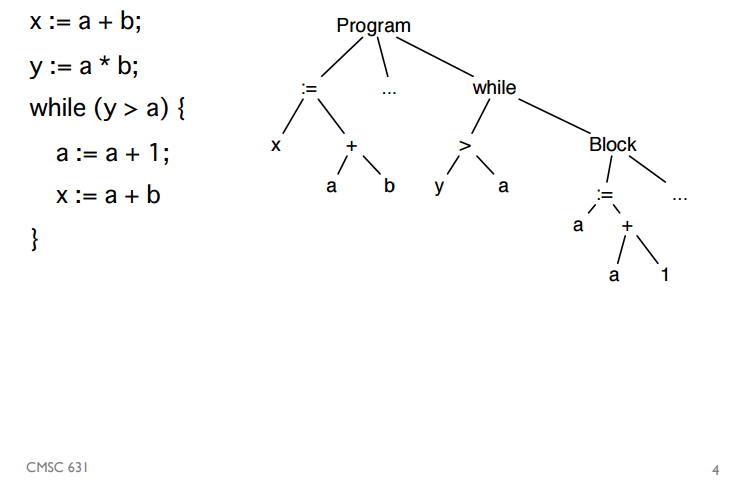
\includegraphics[width=0.9\textwidth]{image001.png}
\end{center}
\caption{Example of an Abstract Syntax Tree that both PMD and Checkstyle use. \cite{1_foster_2016}.}
\end{figure}

 